
\section{Theorie}
\label{sec:Theorie}
\subsection{Brechungsindex und Reflexion}
\label{sec:Brechungsindex}
Beim Auftreffen von Röntgenstrahlung vom Vakuum auf ein Medium, dessen Brechungsindex von eins abweicht, ist gegeben durch:
\begin{equation}
  \label{eqn:Brechungsindex}
  n=1-\delta+ i\cdot \beta
\end{equation}
$\beta$ ist dabei die Absorption und $\delta$ ist ein Korrektur. Bei Röntgenstrahlung ist bei diesem Übergang eine Totalreflexion möglich, da der Brechungsindex in Materie kleiner als Eins ist. Im allgemeinen Fall trifft die elektromagnetische Welle in einem Winkel $\alpha_\mathrm{e}$ auf eine unendlich dicke, homogene, glatte Materialschicht. Ein Teil wird dann im Winkel $\alpha_\mathrm{e}=\alpha_\mathrm{r}$ reflektiert. Der restliche Teil wird unter dem Winkel $\alpha_\mathrm{t}$ gebrochen und transmittiert. Die Totalreflexion tritt hierbei unter dem kritischen Winkel $\alpha_\mathrm{c}$ auf. Dies bedeutet, dass keine Transmission auftritt. Dieser Kritische Winkel beim Auftreffen von Röntgenstrahlung vom Vakuum auf ein Medium, dessen Brechungsindex von eins abweicht, ist gegeben durch:
\begin{align}
  \label{eqn:Totalreflexion}
  a_\mathrm{c} &= \sqrt{2 \delta} \\
  a_\mathrm{c} &= \lambda\cdot\sqrt{\dfrac{r_\mathrm{e}\cdot\rho}{\pi}}
\end{align}
Die Fresnelschen-Gleichungen beschrieben die Reflexion und Transmission an ebenen Grenzschichten. Die Polarisation kann aufgrund des Sonderfalles, dass die magnetischen Permeabilitäten ungefähr gleich groß sind, vernachlässigt werden. Die Gleichungen vereinfachen sich so zu:
\begin{align}
  \label{eqn:Fresnelschen-Gleichungenl}
  t &= \dfrac{2\cdot n_\mathrm{1} \sin(\alpha_\mathrm{e}) }{n_\mathrm{1} \sin(\alpha_\mathrm{e})+ n_\mathrm{2} \sin(\alpha_\mathrm{c})}\\
  r &= \dfrac{n_\mathrm{1} \sin(\alpha_\mathrm{e})-n_\mathrm{2}\sin(\alpha_\mathrm{c})}{n_\mathrm{1}\sin(\alpha_\mathrm{e})+n_\mathrm{2} \sin(\alpha_\mathrm{c})}
\end{align}
$r$ und $t$ beschrieben dabei die Fresnel`schen Reflexions- und Transmissionskoeffizienten. Diese beschreiben die Amplitudenverhältnisse. Die Intensitätsverhältnisse können über die Fresnel`sche Reflektivität mit der Annahme, dass $\alpha_\mathrm{e} >3 \alpha_\mathrm{c}$ als:
\begin{equation}
  \label{eqn:Fresnelref}
 R_\mathrm{F} =|r|^2 =\left(\dfrac{\alpha_\mathrm{c}}{2\alpha_\mathrm{e}}\right)^4
\end{equation}
beschrieben werden.
\subsection{Mehrschichtensysteme}
\label{sec:Mehrschichtensysteme}
Die Systeme  sind in der Realität bestehen meist nicht aus nur einer Schicht und sind auch nicht homogen. Als erstes wird die Reflexion an einer nicht homogenen Schicht untersucht, hier an einer  dicken Polystyrolschicht mit einer Dicke von $\SI{80}{\nano\meter}$. Wenn nun die Reflektivität gegen den Einfallswinkel aufgetragen wird, ergibt sich:
\begin{figure}[h!]
  \label{fig:kiessig}
  \centering
  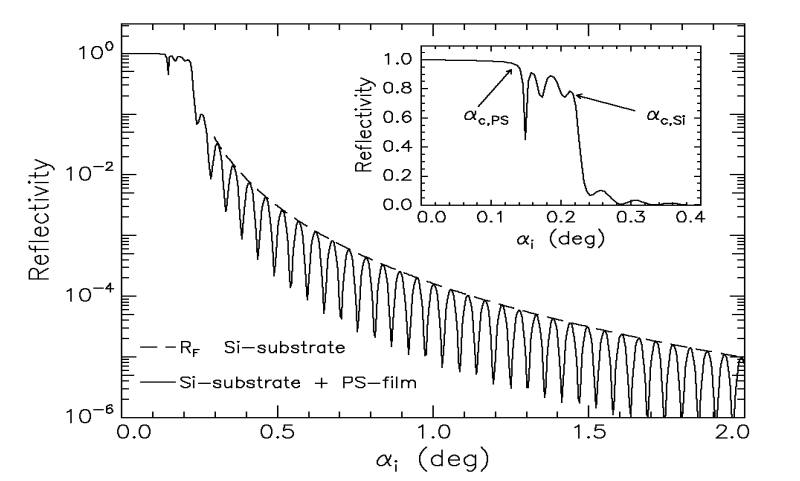
\includegraphics[scale=0.4]{fig/kiessing.png}
  \caption{Reflektivität eines Siliziumwafers mit einer $\SI{80}{\nano\meter}$ dicken Polystyrolschicht \cite[8]{Anleitung3}}
\end{figure}
\FloatBarrier
\noindent Die theoretische Fresenelreflektivität wird dabei als gestrichelte Linie dargstellt. In der Realität oszilliert die Reflektivität, dies wird als Kiessig-Oszillation bezeichnet. Diese entstehen durch Interferenzen an den Grenzschichten, die je nach Phasendifferenz konstruktiv oder destruktiv sind. Die Minima entstehen bei einem Gangunterschied vpn $N\cdot\dfrac{\lambda}{2}$, wobei N eine ungerade Zahl ist. Bei den kritischen Winkel $\alpha_\mathrm{c}$ sind Einbrüche im Plot zu finden, wodurch diese bestimmt werden können. Die Schichtdicke kann über die Ozillation und die Wellenlänge $\lambda$ bestimmt werden als:
\begin{equation}
  \label{eqn:Schichtdicke}
d = \dfrac{\lambda}{2\Delta a_\mathrm{i}}
\end{equation}
wobei $d$ die Schichtdicke ist und  $a_\mathrm{i}$ der Winkel zwischen zwei Minima der Kiessig-Oszillation ist.
Wenn nun weitere Schichten hinzukommen, werden sich die Oszillationen der einzelnen Schichten überlagern. Um dennoch etwas über die Reflektivität aussagen zu können, wird der Parratt-Algorithmus verwendet. Dieser besteht aus dem rekursiven Durchlaufen aller Schichten, angefangen von der untersten Schicht. Dabei wird die jeweils j-te Schicht und deren Amplitudenverhältnisse untersucht. Dabei ist der Parratt-Algorithmus gegeben durch:
\begin{align}
  \label{eqn:Parratt-Algorithmus}
X_\mathrm{j}= \exp(-2i k_\mathrm{z,j}z_\mathrm{j})\cdot\dfrac{r_\mathrm{j,j+1}+X_\mathrm{j}\exp(-2i k_\mathrm{z,j+1}z_\mathrm{j})}{1+r_\mathrm{j,j+1}+X_\mathrm{j}\exp(-2i k_\mathrm{z,j+1}z_\mathrm{j})}
\end{align}
Hierbei ist
\begin{equation}
  \label{eqn:kzj}
 k_\mathrm{z,j}= k\cdot\sqrt{n_\mathrm{j}^2-(\cos(\alpha_\mathrm{i})^2}
\end{equation}
die z-Komponente des j-ten Wellenvektors. Der Betrag ist dabei $k=\dfrac{2\pi}{\lambda}$. Die Fresnelkoeffizienten werden dann über
\begin{equation}
  \label{eqn:Veränderten Fresnelkoefizienten}
  r_\mathrm{j,j+1}= \dfrac{k_\mathrm{z,j}-k_\mathrm{z,j+1}}{ k_\mathrm{z,j}+ k_\mathrm{z,j+1}}
\end{equation}
berechnet.
\subsection{Rauigkeit}
\label{sec:Rauigkeit}
Die nächste Korektur ist die der Rauigkeit. Glatte Materialschichten sind in der Realität nicht anzutreffen, weshalb die Rauigkeit der j-ten Grenzfläche eingeführt wird. Dies ist gegeben durch:
\begin{equation}
  \label{eqn:rms}
\sigma_\mathrm{j}^2= \int (z-z_\mathrm{j})\cdot P_\mathrm{j}(z) dz.
\end{equation}
$P_\mathrm{j}(z)$ ist dabei die Wahrscheinlichkeit des Antrefens der j-ten Grenzfläche im Intervall $(z_\mathrm{j}+z,z_\mathrm{j}+z+dz)$.
Damir werden die Fresnelkoeffizienten zu:
\begin{align}
  \label{eqn:modkoeff}
  \overline{r}_\mathrm{j,j+1}&=r_\mathrm{j,j+1}\cdot\exp(-2 k_\mathrm{z,j} k_\mathrm{z,j+1}\sigma_\mathrm{j}^2) \\
  \label{eqn:modkoeff2}
  \overline{t}_\mathrm{j,j+1}&=t_\mathrm{j,j+1}\cdot\exp\left(( k_\mathrm{z,j}-k_\mathrm{z,j+1})^2 \dfrac{\sigma_\mathrm{j}^2}{2}\right)
\end{align}
Diese modifizierten können im Parratt-Algorithmus verwendert werden.
\subsection{Funktionsweise der Geräte}
\label{sec:Geräte}
Für die Röntgenstrahlung wird eine Kupfer-Röntgenröhre verwendet. Elektronen werden zu einer Kupfer-Anode beschleunigt. Dort wird Bremstrahlung abgegeben und durch Stoßprozesse mit den Hüllenelektronen entstehen die charakteristische Strahlung, wobei die $K_\mathrm{\alpha}$-Linie für diesen Veruch verwendet wird. Um nur diese für die Reflektometrie zu verwenden, wird ein Göbelspiegel benutzt. Dieser bündelt die Strahlen, sodass diese monochromatisiert werden und parallel verlaufen. Die Wellenlänge, die durch gelassen wird, beträgt $\lambda=\SI{1.54 e-10}{\meter}$ und entspricht der $K_\mathrm{\alpha}$-Linie.
Bei dem Versuch defnieren zwei Blenden jewils den Einfallswinkel und den Ausfalsswinkel. Eine zusätzliche Bedingung ist, dass erst ab einem Geometrie-Winkel $\alpha_\mathrm{g}$ der gesamte Strahl reflektiert wird. Dieser Winkel lässt sich über
\begin{equation}
  \label{eqn:Geometriewinkel}
a_\mathrm{g}=\arcsin\left(\dfrac{d_\mathrm{0}}{D}\right)
\end{equation}
berechnen. Dabei ist $d_\mathrm{0}$ die Gesamtstrahlbreite und $D$ die Probelänge. Mit der tatsächlichen Strahlbreite $D\cdot\sin(\alpha_\mathrm{e})$, die auf die Probe trifft lässt sich der Geometriefaktor G als
\begin{align}
  \label{eqn:Geometriefaktorl}
G= \dfrac{D\cdot\sin(\alpha_\mathrm{e})}{d_\mathrm{0}}
\end{align}
im Bereich $ \alpha_\mathrm{e}< \alpha_\mathrm{g}$ bestimmen. Für den Bereich $\alpha_\mathrm{e}\geq\ \alpha_\mathrm{g}$ beträgt der Geometriefaktor $G=1$.
